\documentclass{beamer}

\usetheme{default}
%\usetheme{Warsaw} %%% we will try Warsaw as well
%\usetheme{Berkeley} %%% some themes such as this one will display your section/subsection categories

\title{My Awesome Presentation}
\subtitle{Simple Beamer}
\author{Student}
\date{\today}

\begin{document}

\begin{frame}
  \titlepage
\end{frame}

\section{Introduction}
%%%%%%%%%%%% Slide %%%%%%%%%%%%%%%%%%%%%%%%%%%%%%%%%%%%%%%%%%%%%%%%%%%
\begin{frame}
  \frametitle{Styles}
  We are using the default theme, but you can find various pre-defined Beamer styles here: \\
 	$http://www.hartwork.org/beamer-theme-matrix/$
 	
 \noindent Check out wikibooks on more information about the Beamer \\
 $http://en.wikibooks.org/wiki/LaTeX/Presentations$
\end{frame}
%%%%%%%%%%%% Slide %%%%%%%%%%%%%%%%%%%%%%%%%%%%%%%%%%%%%%%%%%%%%%%%%%%
\subsection{Lists}
\begin{frame}
  \frametitle{Itemized lists}
 	\begin{itemize}
        \item One item
        \item Two items
        \item More items
    \end{itemize}
\end{frame}
%%%%%%%%%%%% Slide %%%%%%%%%%%%%%%%%%%%%%%%%%%%%%%%%%%%%%%%%%%%%%%%%%%
\begin{frame}
  \frametitle{Enumerated lists}
	\begin{enumerate}
        \item Very similar to itemized list
        \item Only using numbers instead of bullets
    \end{enumerate}
\end{frame}
%%%%%%%%%%%% Slide %%%%%%%%%%%%%%%%%%%%%%%%%%%%%%%%%%%%%%%%%%%%%%%%%%%
\subsection{Math}
\begin{frame}
  \frametitle{I can do pretty math!}
	\begin{equation}
	y = 2x + 3
	\end{equation}
    \begin{theorem}
  		In a right triangle, the square of hypotenuse equals
  		the sum of squares of two other sides.
	\end{theorem}

\end{frame}
%%%%%%%%%%%% Slide %%%%%%%%%%%%%%%%%%%%%%%%%%%%%%%%%%%%%%%%%%%%%%%%%%%
\begin{frame}
  \frametitle{Tables}
  \begin{center}
	\begin{tabular}{|c|c|}
		\hline 
        \textbf{Description} & \textbf{Order of growth} \\
        \hline 
        Constant & $1$ \\
        Logarithmic & $log N$ \\
        Linear & $N$ \\
        Linearithmic & $N log N$ \\
        Quadratic & $N^2$ \\
        Cubic & $N^3$ \\
        Exponential & $2^N$\\
        \hline
    \end{tabular}
    \end{center}
\end{frame}
%%%%%%%%%%%% Slide %%%%%%%%%%%%%%%%%%%%%%%%%%%%%%%%%%%%%%%%%%%%%%%%%%%
\section{More things}
\subsection{Blocks}
\begin{frame}
  \frametitle{Blocks}
    \begin{alertblock}{More precise definition}
    Given two nonnegative functions $f$ and $g$, $f(N)$ is  $O(g(N))$ iff $\exists$ constant $c > 0$ so that $f(N) \leq c g(N)$
    \end{alertblock}
\end{frame}
%%%%%%%%%%%% Slide %%%%%%%%%%%%%%%%%%%%%%%%%%%%%%%%%%%%%%%%%%%%%%%%%%%
\begin{frame}[label=Flower]
  \frametitle{Image}
    \begin{center}
        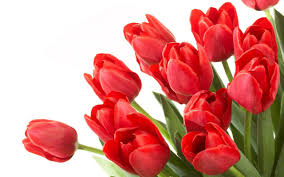
\includegraphics[width=3in]{images/flower.jpeg}
    \end{center}
    \hyperlink{Overlays}{\beamerbutton{Overlays}}
\end{frame}
%%%%%%%%%%%% Slide %%%%%%%%%%%%%%%%%%%%%%%%%%%%%%%%%%%%%%%%%%%%%%%%%%%
\subsection{Overlays}
\begin{frame}
  \frametitle{Pause}
  \pause
 	\begin{itemize}
        \item Sometimes
        \pause
        \item it is nice
        \pause
        \item to pause
    \end{itemize}
\end{frame}
%%%%%%%%%%%% Slide %%%%%%%%%%%%%%%%%%%%%%%%%%%%%%%%%%%%%%%%%%%%%%%%%%%
\begin{frame}[label=Overlays]
  \frametitle{Overlays}

	\setbeamercovered{transparent}
    \begin{itemize}
        \item<1-> One item
        \item<2-> at a 
        \item<3-> time
    \end{itemize}
    \hyperlink{Flower}{\beamerbutton{Flower}}
\end{frame}
%%%%%%%%%%%% Slide %%%%%%%%%%%%%%%%%%%%%%%%%%%%%%%%%%%%%%%%%%%%%%%%%%%
\section{Conclusion}
\begin{frame}
\begin{center}
\Huge
 Thank You!

Questions?

\vspace{0.2in}

\normalsize

\href{mailto:student@allegheny.edu}{\color{black}{\texttt{student@allegheny.edu}}}

\vspace{0.1in}

\href{http://cs.allegheny.edu/}{\color{blue}{\texttt{Student\\ http://cs.allegheny.edu/$\sim$ Student}}}

\end{center}
\end{frame}


\end{document}
